
\documentclass[12pt,notitlepage]{article}
%%%%%%%%%%%%%%%%%%%%%%%%%%%%%%%%%%%%%%%%%%%%%%%%%%%%%%%%%%%%%%%%%%%%%%%%%%%%%%%%%%%%%%%%%%%%%%%%%%%%%%%%%%%%%%%%%%%%%%%%%%%%%%%%%%%%%%%%%%%%%%%%%%%%%%%%%%%%%%%%%%%%%%%%%%%%%%%%%%%%%%%%%%%%%%%%%%%%%%%%%%%%%%%%%%%%%%%%%%%%%%%%%%%%%%%%%%%%%%%%%%%%%%%%%%%%
\usepackage{amssymb}
\usepackage{amsmath}
\usepackage{pdfpages}
\usepackage{marvosym}
\usepackage{hyperref}
\usepackage{enumitem}
\usepackage{tikz}
\usepackage{graphicx}
\usepackage{float}

\usepackage{multirow}

\setcounter{MaxMatrixCols}{10}
%TCIDATA{OutputFilter=LATEX.DLL}
%TCIDATA{Version=5.00.0.2552}
%TCIDATA{<META NAME="SaveForMode" CONTENT="1">}
%TCIDATA{LastRevised=Wednesday, February 16, 2011 02:52:30}
%TCIDATA{<META NAME="GraphicsSave" CONTENT="32">}
%TCIDATA{Language=American English}

\topmargin=-1.8cm \textheight=23.8cm \oddsidemargin=-0.3cm
\evensidemargin=-0.5cm \textwidth=17.1cm
\newtheorem{ass}{Assumption}
\newtheorem{prop}{Proposition}
\newtheorem{thm}{Theorem}
\newtheorem{lem}{Lemma}
\newtheorem{conj}{Conjecture}

\begin{document}


\thispagestyle{empty}\baselineskip1.2\baselineskip\

\noindent \textbf{Econ 140\newline
Summer 2022 \newline
Instructor: Fernando Hoces de la Guardia \newline
GSIs: Elena Stacy \& Yige Wang
}

\vskip2ex

\noindent \textbf{Midterm Exam 1}

\vskip3ex

\noindent \textbf{Thursday July 7, 2022}

\vskip9ex

\vskip9ex


\noindent \textbf{Exam Instructions:}


\begin{itemize}
\item \textbf{You have 80 minutes to answer this exam} 

\item \textbf{This exams has a total of 80 points (suggesting the length of time to spent in each question). Each question indicates the number of points, and indicates a maximum length for its answer} 

\item \textbf{Most questions ask for short answers (from a couple of words, to one or two sentence maximum)} 
\item \textbf{Explanation in black or blue ink is recommended as these often scan the best.} 
\item \textbf{You must submit your solutions using the exam packet provided.} 
\item \textbf{Do not write your solutions on pages that say ``Do not write solutions on this page"}. Answers written on these pages will not be graded. You may use these pages as scratch paper.
\item \textbf{When time is called, STOP} writing, immediately \textbf{CLOSE} your exam packet and hold it up until it is collected.
\item \textbf{Show your work}. Credit will only be awarded on the basis of what is written on the exam.
\item \textbf{Sign the academic honesty pledge}. Cheating will be punished.
\end{itemize}

\newpage

\vspace{2.5in}

\noindent Student Name:

\vskip5ex

\noindent Student ID Number:

\vskip10ex

\noindent \textbf{Affirm the academic honesty pledge below}. For those writing on a non-printed copy, please just write ``Academic Honesty Pledge as on exam'', and sign your name. \\\textbf{\underline{If you do not affirm this pledge, your exam will be marked invalid.}}


\vskip12ex

\noindent \textbf{0. ACADEMIC HONESTY PLEDGE }

\noindent I confirm that I have abided by all academic honesty rules for UC Berkeley and Economics 140. I confirm that I did not see this exam before my official exam start time. I confirm that I have not shared and will not share this exam with anyone else. I confirm that I haven't copied from anybody else's exam.

\vskip5ex

Signature: \hrulefill

\vskip5ex


\newpage

%\noindent \textbf{1. Short Questions (15 points, 3 points per question.)}

\vskip1ex

\begin{enumerate}

	\item  Based on our class discussion of the concept of bullshit: what is the key characteristic that distinguishes bullshit from lies (or the bullshitier from the liar) [2pt, 1-2 sentences].   
	




\vspace{3cm}



	\item How can we compute the probability of an event for the case of a continuous random variable? [2pt, 1 sentence] 
	
\vspace{3cm}

	\item For the case of a continuous random variable: which distribution is a good representation of not knowing much about a phenomenon (represented by the random variable)? How about for a discrete random variable (assume 2 events for simplicity)?
	[2pt, 2 sentences]

\vspace{3cm}

\item 
    The probability that two random variables, $X, Y$ take the values of $x$, \textbf{and} $y$ can \textbf{always} be described as: [2pt]
    \begin{enumerate}[label=\alph*)]
    \item  $\operatorname{Pr}(\mathrm{X}=\mathrm{x})+(\mathrm{Y}=\mathrm{y})$
    \item $\operatorname{Pr}(\mathrm{X}=\mathrm{x}, \mathrm{Y}=\mathrm{y})$.
    \item $\operatorname{Pr}(\mathrm{X}=\mathrm{x}) *(\mathrm{Y}=\mathrm{y})$
    \item $\operatorname{Pr}(\mathrm{X}=\mathrm{x}) /(\mathrm{Y}=\mathrm{y})$
    \end{enumerate}
 \vspace{1cm}
\item Using the concept of conditional probabilities, the same term as in the question above (the probability that two random variables, $\mathrm{X}, \mathrm{Y}$ take the values of $\mathrm{x}$, and $\mathrm{y})$ can be described as. [2pt]
\begin{enumerate}[label=\alph*)]
    \item $\operatorname{Pr}(\mathrm{X}=\mathrm{x} \mid \mathrm{Y}=\mathrm{y})^{*} \operatorname{Pr}(\mathrm{X}=\mathrm{x})$
    \item $\operatorname{Pr}(\mathrm{Y}=\mathrm{y} \mid \mathrm{X}=\mathrm{x})^{*} \operatorname{Pr}(\mathrm{Y}=\mathrm{y})$
    \item $\operatorname{Pr}(\mathrm{X}=\mathrm{x} \mid \mathrm{Y}=\mathrm{y})^{*} \operatorname{Pr}(\mathrm{Y}=\mathrm{y})$
    \item $\operatorname{Pr}(\mathrm{Y}=\mathrm{y} \mid \mathrm{X}=\mathrm{X})$
\end{enumerate}

\vspace{1cm}


\item Define the concept of independence in plain English [4pt, 1-2 sentences]
    \vspace{3cm}
    \item Define the concept of independence in terms of conditional probabilities. [2pt, 1-2 sentences equation] 
     \vspace{3cm}


\vspace{3cm}

	\item In which sense is the variance, an average. What is an average of? [2pt, 1 sentence]
	
\vspace{3cm}

	\item Compute the variance for a variable with values 2,3, and 4. Show your calculations. [4pts, 2-5 lines] 

	
\vspace{5cm}
\newpage
	\item An econometrics class has 75 students, and the mean student weight is 155 lb. A random sample of four students is selected from the class, and their average weight is calculated. 
	\begin{enumerate}
	    \item Will the average weight of the students in the sample equal 155 lb? [1pt, Yes/No] 
	    \vspace{2cm}
	    \item Explain why you answered yes or no to the above question. [1pt, 1 sentence] 
	    \vspace{2cm}
	    \item Is the sample average, $\overline{Y}$ , a random variable? [1pt, 1 sentence] 
	\end{enumerate}

\vspace{3cm}

	\item In a rectangular data set: what is represented by rows and what by columns.  [1pt, 1 sentence]
	\vspace{3cm}
	\item Assume that you have received a data set with millions of observations on the income of all the American households. Which concept(s) discussed in class can you use to communicate some initial insights about these millions of observations? [2pt, 1 sentence]
	\vspace{3cm}
	\item What is the interpretation of the mean of a binary variable? [2pt, 1 sentence]
	\vspace{3cm}

\newpage
	\item What is the main reason we prefer to report (and read) standard deviations instead of variances? [2pt, 1 sentence]
\vspace{3cm}
	\item Given a collection of random variables, Y1, Y2, …, Yn let $\overline{Y}$ represent its sample mean. What happens with its expected value as the number of random (n) variables increases. What happens to its variance? [2pt, 1-2 sentences]
\vspace{3cm}
	
\item Given a data set with information on the age of each individual in the US (360 million), choose which of the following could be a \textbf{plausible} value for the standard deviation\textbf{ of the sample mean}. [2pt]
\begin{enumerate}
    \item -32
    \item 32
    \item 320
    \item 0.32
\end{enumerate}
\vspace{1cm}

\item Explain your answer to the above question. [2pt, 1 sentence]
\vspace{3cm}

\item For the simulation performed in class and sections to explore the Central Limit Theorem: 
\begin{enumerate}
    \item What happens with the distribution of the sample mean as we increase the sample size? [4pt, 1-2 sentences]
    \vspace{3cm}
    \item What happens with the distribution as we increase the number of simulations/draws? [2pt, 1 sentence]
\end{enumerate}
\vspace{3cm}

\item Name what is the key assumption that is violated when we observe a spurious correlation. [3pt, 1 sentence]
\vspace{3cm}

\item Let’s look again at the table used to explain the intuition behind conditional probabilities. Add two new variables “$Pass|S=1$” and “$Pass \text{ \& } S$” and fill-in the corresponding value of each observation [2 columns, 6pts]. 
\begin{figure}[H]
    \centering
    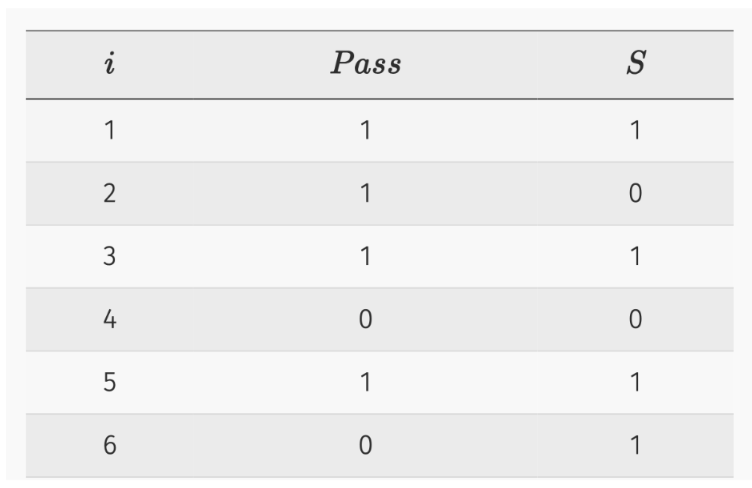
\includegraphics[width=4in]{Figures/midterm_pass.png}
    \caption{}
    \label{}
\end{figure}
\vspace{5cm}


\item (Modified ``Conditionities''). Annie lives in a town of 3000 individuals where a disease called "Conditionities" is scaring the population. The disease affects 2\% of the population and there is a test that detects the disease with 90\% success (meaning that, when a person has the disease, the tests comes positive 90\% of the time; and when the person does not have the disease, it comes negative 90\% of the time). Annie just took a test and it came up positive, what is the probability that the has the disease? [6pt, 2-6 lines] 

[Suggestion: getting stuck in this question might consume a significant portion of your time, if the answer doesn't come to you immediately, leave it for the end]

[Help, in addition to Bayes formula printed on question 27, you might also need the law of total probabilities. This states that for two random variables X and Y, the probability of X taking a specific value can be broken down into the following conditional probabilities:]

\begin{equation}
    P(X=x) = \sum_{i}P(X=x|Y=y_i)P(Y=y_i)
\end{equation}


\vspace{3cm}

\item Describe the intuition behind balance in pre-treatment variables. [4pt, 1-3 sentences] 
\vspace{3cm}


\item Provide a one-line interpretation for all the numbers highlighted in the 2rd row of the following table (one line per box)? [8pt, 3 sentences] 
\begin{figure}[H]
    \centering
    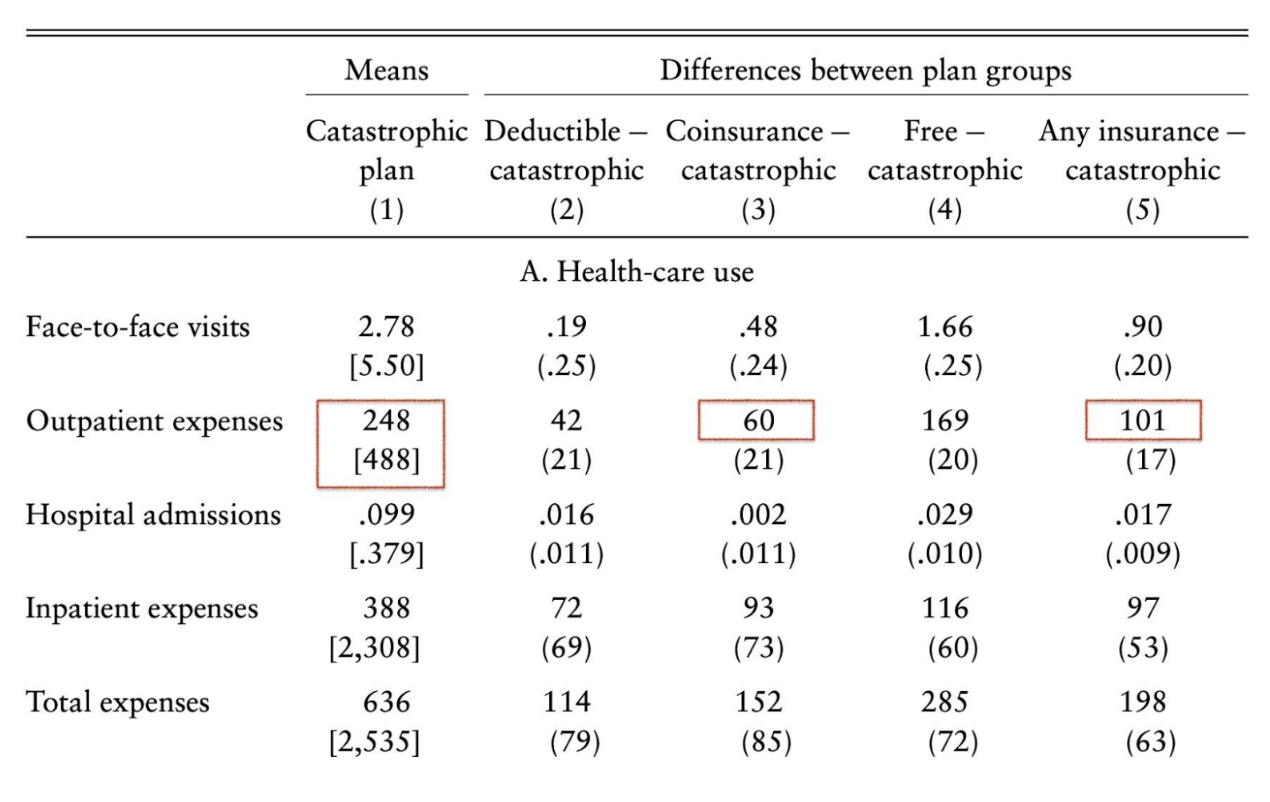
\includegraphics[width=6in]{Figures/midterm_table.png}
    \caption{}
    \label{}
\end{figure}
\vspace{2cm}

\item For the exercise of potential outcomes done in class with a fictional data of 10 individuals, cross with an x the potential outcomes that are missing from the data. [6pts, write x's on table] 
\begin{figure}[H]
    \centering
    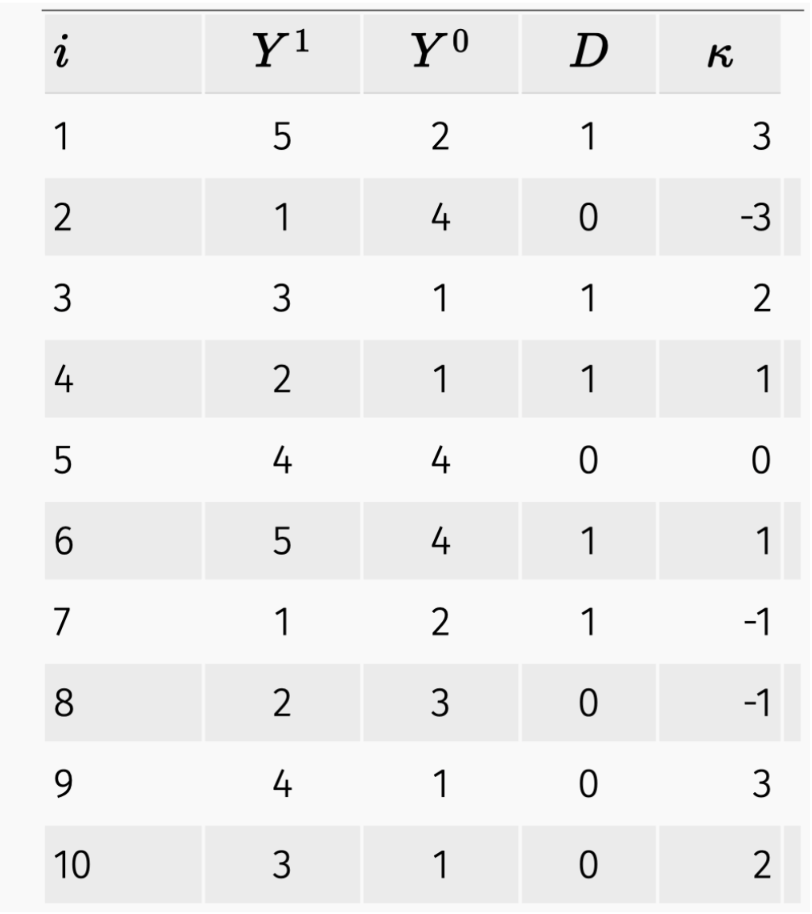
\includegraphics[width=3in]{Figures/midterm_outcome.png}
    \caption{}
    \label{}
\end{figure}
\vspace{3cm}


\item $\mathbb{V}(Y)=\mathbb{E}(\mathbb{V}(Y \mid X))+\mathbb{V}(\mathbb{E}(Y \mid X))$

Ev(v)es Law, the expression above, tells us that the unconditional variance will always be [3pt] : 
\begin{enumerate}
    \item Larger or equal than the conditional variance
    \item Smaller or equal than the conditional variance
    \item Larger when the Y is independent of X
    \item Smaller when Y is independent of X
\end{enumerate}
\vspace{3cm}
\newpage

\item \textit{[Bonus Question. Suggestion: focus on this question only after you are done with the rest of the exam]}

Monty Hall Problem (slightly modified):
Suppose you're on a game show, and you're given the choice of \textbf{four} doors: Behind one door is a car; behind the others, goats. You pick a door, say No. 1, and the host, \textbf{who knows what's behind the doors}, opens another door, say No. 4, which has a goat. He then says to you, "Do you want to pick door No. 4?" Is it to your advantage to switch your choice?

Explain the solution to the Monty Hall problem in plain English.[3pts, 1-3 sentences]
\vspace{3cm}

\item $[Bonus]$ Derive the solution to the Monty Hall problem using Bayes rule [3pts, 2-6 lines]. 
Reminder of Bayes rule 
\begin{equation}
    P(A|B) = \frac{P(B|A)P(A)}{P(B)}
\end{equation}
\vspace{3cm}



\newpage
\begin{center}
	\noindent{[Do not write on this page.]}
\end{center}
\newpage

\newpage
\begin{center}
	\noindent{[Do not write on this page.]}
\end{center}
\newpage
\end{enumerate}




\end{document}
